\documentclass[11pt,a4paper]{article}
\usepackage[margin=25mm]{geometry}
\usepackage{amsmath,amssymb,booktabs,graphicx,hyperref,placeins}
\usepackage{xcolor}
\graphicspath{{../results/experiment_0/}{../results/experiment_1/}{../results/experiment_2/}{../results/experiment_3/}{../results/experiment_4/}{../results/experiment_5/}{../results/pilot_p1/}{../results/pilot_p2/}{../results/pilot_p3/}}
\hypersetup{colorlinks=true,linkcolor=blue,urlcolor=blue,citecolor=blue}

\title{Building Utility Twin\\\large Simulation Framework, Experiments, and Pilot Preparation}
\author{Jakob Weber}
\date{\today}

\begin{document}
\maketitle
\tableofcontents

\section{Purpose and scope}
The Building Utility Twin is a simulation-first framework for developing the
interfaces, data contracts, storage layer, and validation logic required by a
real building-utility application. The central engineering principle is that
simulated and physical assets expose the same canonical measurements. Replacing
a simulator with a device adapter should therefore not require changes to the
storage, analysis, or reporting layers.

The long-term system covers cold water, domestic hot water, the central boiler,
thermal energy, apartments, meter imperfections, and operational anomalies.
Iteration A intentionally starts with a single water pipe. This small vertical
slice is used to validate the architecture before physical and operational
complexity are added. Iteration B then introduces the first physically meaningful
coupling: domestic hot-water consumption supplied by a central boiler.
Iteration C keeps that physical reference fixed and tests the meter and
communications boundary under realistic data-path imperfections.
Iteration D expands the topology to multiple apartments and replaces the
instantaneous boiler with a dynamic shared domestic-hot-water store.
Iteration E composes this building with imperfect meter telemetry and adds the
first operational reconciliation and anomaly-detection layer.
Iteration F exercises the architecture's central substitution claim by replacing
the simulator-facing source with a configurable CSV adapter while retaining the
canonical contract, file store, and water-balance calculation.

\section{System architecture}
The intended data path is
\begin{equation}
  \begin{aligned}
  \text{scenario} &\rightarrow \text{physical simulator}
  \rightarrow \text{virtual meter} \\
  &\rightarrow \text{telemetry transport}
  \rightarrow \text{canonical measurement}
  \rightarrow \text{storage} \rightarrow \text{analysis/report}.
  \end{aligned}
\end{equation}
Every boundary is explicit. The simulator produces physical truth, the meter
models what an instrument reports, the measurement contract gives the report a
stable meaning, and storage persists the contract without domain-specific
reinterpretation.

The canonical timestamp remains the time at which the device observed the
quantity. Transport metadata records reception time separately. This
distinction allows delayed and out-of-order packets to be reordered without
rewriting the physical time semantics of the measurement.

\subsection{Canonical units and sign convention}
Internal calculations use SI units. Volumetric flow rate $q_k$ is in
$\mathrm{m^3\,s^{-1}}$; cumulative volume $V_k$ is in
$\mathrm{m^3}$. Positive flow follows the pipe orientation from inlet to
outlet. Timestamps are timezone-aware UTC values and intervals are interpreted
as half-open intervals $[t_k,t_{k+1})$.

\subsection{Canonical measurement contract}
Each persisted measurement shall contain at least: schema version, unique
measurement identifier, asset identifier, channel, physical quantity,
timestamp, numerical value, canonical unit, quality flag, and source. The
contract validates quantity--unit compatibility and rejects non-finite values,
naive timestamps, and empty identifiers. Its serialization is deterministic so
that experiment outputs can be compared byte-for-byte.

For interval-average flow, an additional duration field defines the integration
interval. A cumulative register is an instantaneous boundary reading and has no
duration. Table~\ref{tab:channels} gives the two Experiment~0 channels.
\begin{table}[htbp]
  \centering
  \caption{Canonical channels used in Experiment~0.}
  \label{tab:channels}
  \begin{tabular}{llll}
    \toprule
    Channel & Asset & Quantity & Unit / time semantics \\
    \midrule
    \texttt{outlet\_flow} & \texttt{pipe-001} & volumetric flow rate
      & $\mathrm{m^3\,s^{-1}}$, 60-s mean \\
    \texttt{cumulative\_register} & \texttt{meter-001} & cumulative volume
      & $\mathrm{m^3}$, boundary value \\
    \bottomrule
  \end{tabular}
\end{table}

\section{Iteration A: minimum vertical slice}
Iteration A establishes an end-to-end implementation with one pipe and no
network branching. Heating is intentionally outside Experiment~0; the next
iteration will use domestic-hot-water flow as the interface to the central
boiler and calculate thermal energy from mass flow and temperature lift.

\subsection{Experiment 0: one pipe, one simulated day}
The simulation covers exactly one UTC day using a fixed time step $\Delta t$.
The pipe is incompressible, has no leak, and stores no varying volume. Its inlet
and outlet flows are therefore identical:
\begin{equation}
  q_{\mathrm{in},k}=q_{\mathrm{out},k}=q_k.
\end{equation}
A seeded stochastic demand scenario generates non-negative, piecewise-constant
flow. A virtual ideal cumulative meter integrates outlet flow:
\begin{equation}
  V_0=0, \qquad V_{k+1}=V_k + q_k\Delta t.
\end{equation}
The end-of-day conservation residual is
\begin{equation}
  r_V = \sum_{k=0}^{N-1}q_{\mathrm{in},k}\Delta t
        -\left(V_N-V_0\right).
\end{equation}
For the ideal configuration, $r_V$ must be zero to numerical precision.

\subsection{Required outputs}
The experiment shall persist canonical measurements in a file-backed store and
export an analysis table and machine-readable summary. The first result figure
shall show (i) flow rate over the day and (ii) cumulative volume from the same
run. All results must record the scenario parameters and random seed.

\subsection{Acceptance criteria}
Experiment~0 is complete when all of the following hold:
\begin{enumerate}
  \item exactly one pipe and one complete day are simulated;
  \item flow and cumulative-volume observations pass the canonical contract;
  \item the virtual meter is monotonic and its increments equal
        $q_k\Delta t$;
  \item file storage round-trips measurements without loss;
  \item inlet volume, outlet volume, and meter delta conserve water within a
        declared numerical tolerance;
  \item repeating a run with the same seed gives identical data and summary;
  \item automated tests pass and the first result figure is generated by the
        experiment runner rather than edited manually.
\end{enumerate}

\section{Experiment 0 implementation}
The implementation uses Python~3.11 or newer and separates the vertical slice
into four responsibilities:
\begin{enumerate}
  \item \texttt{contracts.py} implements the validated Python contract,
        deterministic identifiers, and deterministic JSON serialization;
  \item \texttt{simulation.py} implements the seeded demand scenario, the
        lossless pipe, and the virtual cumulative meter;
  \item \texttt{storage.py} atomically replaces and reads a JSON Lines file of
        canonical measurements; and
  \item \texttt{experiment.py} orchestrates the run, checks the storage
        round-trip and conservation, and writes the analysis artifacts.
\end{enumerate}
A language-neutral JSON Schema in \texttt{schemas/measurement.schema.json}
mirrors the Python validation rules. This is the external interface contract
for future device adapters.

\subsection{Demand scenario and reproducibility}
The configuration is a versioned JSON file. The fixed seed is 20260902, the
simulation starts at 2026-01-15 00:00:00 UTC, and the step is 60 seconds. A
smooth morning/evening profile modulates the event-arrival probability. Seeded
draws determine event duration and flow rate, while a small non-negative base
flow avoids embedding sensor behavior in the physical model. The resulting
flow is piecewise constant over every interval.

Reproducibility is tested by executing the complete runner twice in separate
temporary directories and comparing the canonical measurement stream, analysis
CSV, and JSON summary byte-for-byte. The committed summary additionally records
SHA-256 hashes of both data files.

\subsection{Automated verification}
Eight unit and integration tests cover contract validation, deterministic
identifiers, serialization round-trips, file-backed queries, one-day duration,
meter increments, end-of-day conservation, and repeated-run reproducibility.
All eight tests pass. The conservation threshold is
$\varepsilon_V=10^{-12}\,\mathrm{m^3}$.

\section{Experiment 0 results}
The run contains 1440 one-minute flow intervals and 1441 cumulative-register
boundaries. Persisting both channels produces 2881 canonical observations. The
numerical results are summarized in Table~\ref{tab:results}.

\begin{table}[htbp]
  \centering
  \caption{Experiment~0 results for seed 20260902.}
  \label{tab:results}
  \begin{tabular}{lr}
    \toprule
    Metric & Result \\
    \midrule
    Total metered volume & $777.656\,\mathrm{L}$ \\
    Peak flow & $12.642\,\mathrm{L\,min^{-1}}$ \\
    Active one-minute intervals & 131 of 1440 \\
    Pipe balance residual & $0\,\mathrm{m^3}$ \\
    Meter balance residual & $1.055\times10^{-14}\,\mathrm{m^3}$ \\
    Cumulative register monotonic & yes \\
    Conservation test & pass \\
    \bottomrule
  \end{tabular}
\end{table}

Figure~\ref{fig:experiment0} is generated directly by the experiment runner.
Demand appears as sparse draw events, with more activity during the morning,
midday, and early evening windows encoded by the scenario. Every positive flow
interval creates the corresponding increase in cumulative volume. Flat register
segments coincide with the near-zero base demand.

\begin{figure}[htbp]
  \centering
  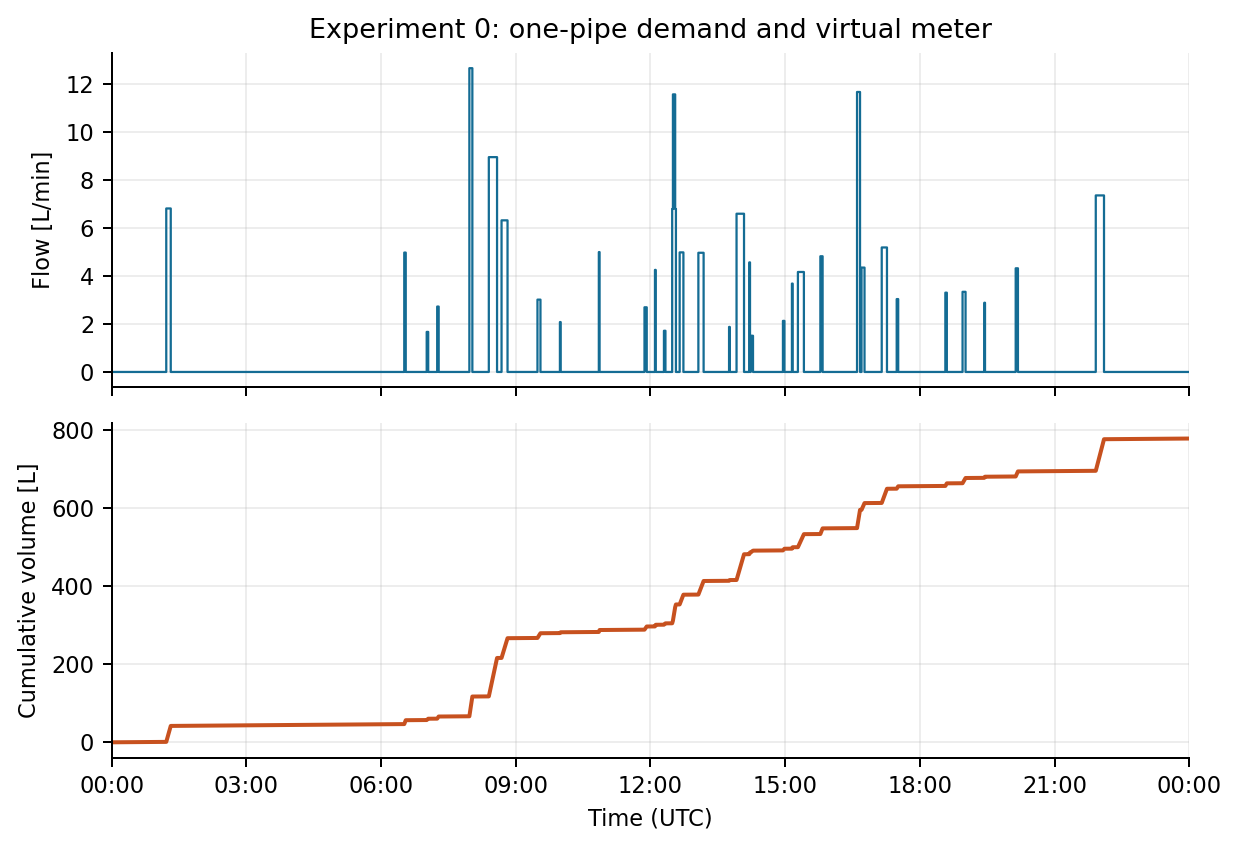
\includegraphics[width=0.96\linewidth]{experiment_0_one_pipe_day.png}
  \caption{One simulated day. Top: outlet flow, equal to inlet flow for the
  lossless one-pipe model. Bottom: the virtual meter's cumulative volume.}
  \label{fig:experiment0}
\end{figure}

The non-zero meter residual is approximately two orders of magnitude below the
declared tolerance and is caused by floating-point summation order: the summary
sums all interval volumes, whereas the meter updates its register sequentially.
The exact zero pipe residual follows from using the same flow at the two pipe
boundaries.

The result validates the software and data path, not household-demand realism.
In particular, $777.656\,\mathrm{L}$ for three synthetic occupants should not be
interpreted as a calibrated daily-use estimate. Before demand behavior is used
for business or engineering conclusions, event frequencies, fixture mixtures,
occupancy, and seasonal effects must be calibrated against field data. This
separation is useful: the contracts, storage, meter semantics, and conservation
tests can now remain fixed while the scenario model is improved.

\section{Iteration B: domestic hot water and central boiler}
Experiment~1 replaces the abstract demand signal with fixture-level events and
introduces cold- and hot-water branches. The goal is not yet a dynamic boiler
model. It is to establish the canonical water--heat interface and verify the
corresponding conservation laws end to end.

\subsection{Reference-day calibration}
An Austrian guidance document reports approximately
$130\,\mathrm{L\,person^{-1}\,day^{-1}}$ total water use, including about
$55\,\mathrm{L}$ of warm water \cite{umweltberatung2016warmwasser}. More recent
klimaaktiv guidance uses approximately $45\,\mathrm{L}$ of warm water per person
and day \cite{klimaaktiv2026dhw}. Experiment~1 therefore defines a transparent
three-person reference day with $130\,\mathrm{L}$ total and $45\,\mathrm{L}$ hot
water per person: $390\,\mathrm{L}$ total, split into $255\,\mathrm{L}$ cold and
$135\,\mathrm{L}$ hot water.

The fixture allocation in Table~\ref{tab:fixtures} is a modelling assumption,
not a measured Austrian end-use distribution. For each fixture, seeded
log-normal weights distribute its fixed daily allocation across events. Seeded
time-profile sampling places events during plausible usage windows. Normalizing
event volumes within each fixture makes the aggregate reference targets exact
while leaving event timing and individual event size stochastic and
reproducible.

\begin{table}[htbp]
  \centering
  \caption{Fixture assumptions and realized event counts for Experiment~1.}
  \label{tab:fixtures}
  \begin{tabular}{lrrrr}
    \toprule
    Fixture & Volume share & Hot fraction & Events & Volume [L] \\
    \midrule
    Toilet & 27\% & 0\% & 18 & 105.3 \\
    Shower & 30\% & 75\% & 3 & 117.0 \\
    Faucet & 23\% & 45\% & 30 & 89.7 \\
    Laundry & 12\% & 0\% & 1 & 46.8 \\
    Dishwasher & 4\% & 0\% & 1 & 15.6 \\
    Cleaning & 4\% & 44.1\% & 3 & 15.6 \\
    \bottomrule
  \end{tabular}
\end{table}

\subsection{Water and energy model}
At every interval the building inlet flow is split without loss:
\begin{equation}
  q_{\mathrm{tot},k}=q_{\mathrm{cold},k}+q_{\mathrm{hot},k}.
\end{equation}
With water density $\rho$, specific heat capacity $c_p$, hot-water flow
$q_{\mathrm{hot},k}$, cold supply temperature $T_{\mathrm{cold}}$, and boiler
supply temperature $T_{\mathrm{hot}}$, useful thermal power is
\begin{equation}
  \dot Q_{\mathrm{use},k} = \rho c_p q_{\mathrm{hot},k}
  \left(T_{\mathrm{hot}}-T_{\mathrm{cold}}\right).
\end{equation}
The ideal boiler has constant efficiency $\eta$, so its input power is
\begin{equation}
  \dot Q_{\mathrm{in},k}=\frac{\dot Q_{\mathrm{use},k}}{\eta}.
\end{equation}
Experiment~1 uses $T_{\mathrm{cold}}=10\,^{\circ}\mathrm{C}$,
$T_{\mathrm{hot}}=60\,^{\circ}\mathrm{C}$, $\rho=997\,\mathrm{kg\,m^{-3}}$,
$c_p=4180\,\mathrm{J\,kg^{-1}\,K^{-1}}$, and $\eta=0.90$. These are explicit
scenario assumptions. The boiler has no storage dynamics, circulation loss,
standby loss, capacity limit, or control transient.

Ideal cumulative meters integrate total, cold, and hot volume as well as useful
and input energy. The canonical contract is extended with temperature in kelvin,
interval-average thermal power in watts, and cumulative energy in joules. The
same JSON Lines storage layer used in Experiment~0 persists all channels.

\subsection{Acceptance criteria and verification}
Experiment~1 is accepted when (i) the configured daily total and hot-water
targets are reproduced, (ii) the water split holds in every interval and for all
cumulative meters, (iii) integrated hot-water energy agrees with the
thermodynamic equation, (iv) useful and input energy agree with the boiler
efficiency, (v) all canonical records survive a file round-trip, and (vi) a
same-seed rerun produces byte-identical measurements, time series, event ledger,
and summary.

The combined suite now contains 17 passing tests. It includes zero-hot-flow,
pointwise water-balance, daily target, thermodynamic energy, efficiency,
contract, meter-integration, storage, and complete repeated-run tests. CI runs
both Experiments~0 and 1 twice and compares their generated data byte-for-byte.

\section{Experiment 1 results}
The seeded reference day contains 56 fixture events and produces 17,285
canonical observations. Table~\ref{tab:experiment1-results} summarizes the main
results.

\begin{table}[htbp]
  \centering
  \caption{Experiment~1 results for seed 20260903.}
  \label{tab:experiment1-results}
  \begin{tabular}{lr}
    \toprule
    Metric & Result \\
    \midrule
    Total / cold / hot volume & 390.000 / 255.000 / 135.000 L \\
    Hot-water share & 34.615\% \\
    Peak total / hot flow & 10.430 / 5.675 $\mathrm{L\,min^{-1}}$ \\
    Peak boiler input power & 21.897 kW \\
    Useful DHW energy & 7.814 kWh \\
    Boiler input energy & 8.682 kWh \\
    Modelled conversion loss & 0.868 kWh \\
    Maximum water-volume residual & $2.50\times10^{-16}\,\mathrm{m^3}$ \\
    Maximum energy residual & $1.86\times10^{-8}\,\mathrm{J}$ \\
    Water and energy conservation & pass \\
    \bottomrule
  \end{tabular}
\end{table}

Figure~\ref{fig:experiment1} shows the complete coupled result. Cold-only
fixtures create no thermal demand. Hot-water portions of shower, faucet, and
cleaning events generate simultaneous boiler-power pulses. The cumulative
volume curves close at their configured targets, while cumulative input energy
ends at $8.682\,\mathrm{kWh}$.

\begin{figure}[htbp]
  \centering
  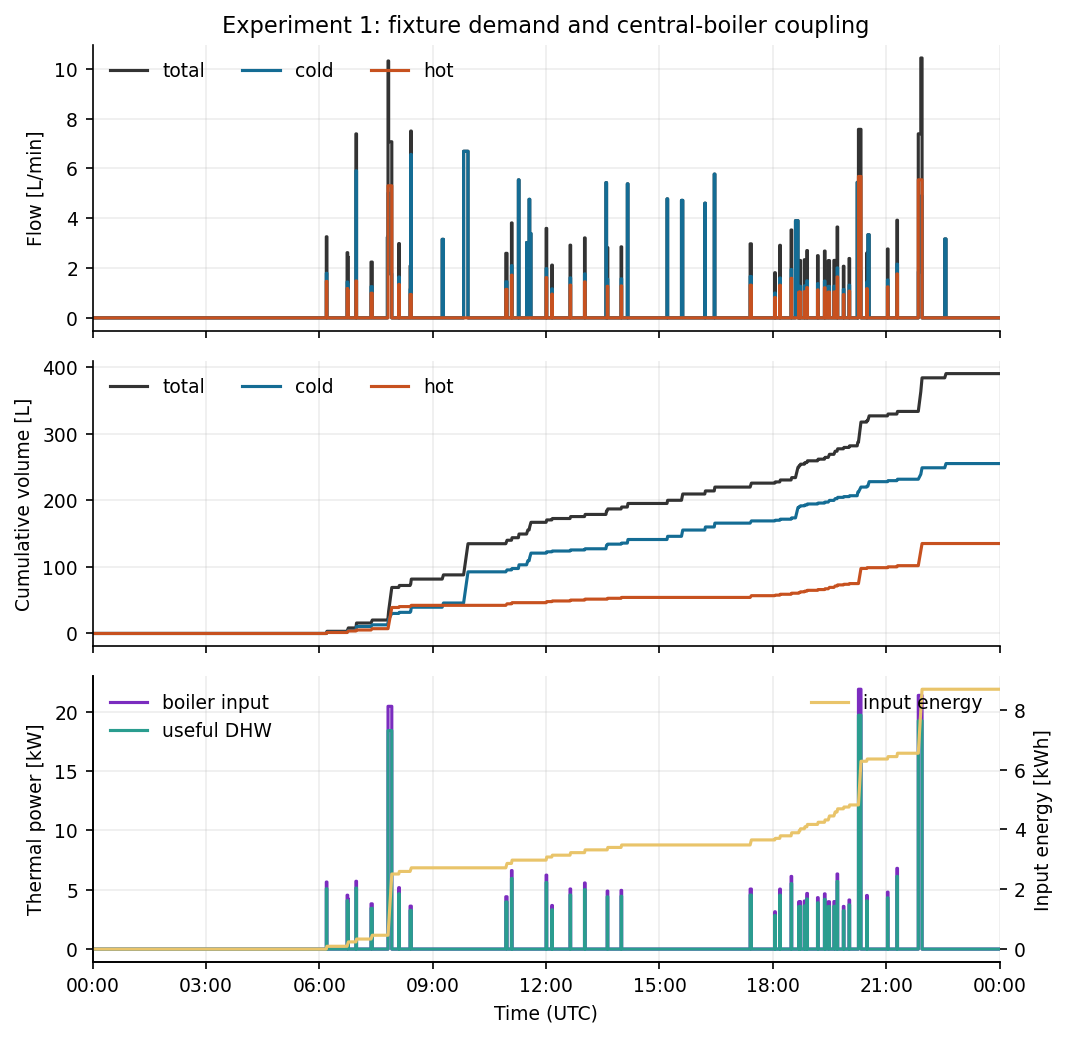
\includegraphics[width=0.86\linewidth]{experiment_1_hot_water_boiler.png}
  \caption{Experiment~1. Top: total, cold, and hot fixture demand. Middle:
  corresponding cumulative volumes. Bottom: useful and boiler-input thermal
  power with cumulative boiler-input energy.}
  \label{fig:experiment1}
\end{figure}

The useful energy of $7.814\,\mathrm{kWh}$ corresponds to approximately
$2.605\,\mathrm{kWh}$ per person for this day. Annualizing only this deliberately
stationary reference calculation gives approximately $951\,\mathrm{kWh}$ useful
energy per person, close to the order-of-magnitude value of
$1000\,\mathrm{kWh}$ reported with the Austrian warm-water guidance
\cite{umweltberatung2016warmwasser}. This is a consistency check rather than an
independent validation because both calculations use comparable daily-volume
assumptions.

The strongest remaining limitation is now explicit: aggregate daily quantities
are calibrated, but fixture shares, within-day timing, and event-size
distributions are assumed. The exact daily totals are useful for isolating and
testing the water--energy interface, but they suppress day-to-day consumption
variability. Moreover, the current boiler transforms hot-water flow into power
instantaneously. It cannot yet represent storage-tank temperature, reheating,
recirculation, standby losses, capacity saturation, or the distinction between
useful tenant energy and plant input over delayed time scales.

\section{Iteration C: imperfect meter and telemetry}
Experiment~2 preserves the exact Experiment~1 physical reference and perturbs
only the total-water meter and its communication path. This separation provides
a known cumulative-volume truth against which ingestion and register recovery
can be tested. It also exercises the same canonical contract and file store that
a later field-device adapter will use.

\subsection{Meter and communication fault model}
For a positive true interval increment $\Delta V_k$, the device integrates
\begin{equation}
  \Delta \widetilde V_k =
  \max\left(0,\Delta V_k(1+\epsilon_k)\right),\qquad
  \epsilon_k\sim\mathcal{N}(0,\sigma^2),
\end{equation}
with $\sigma=0.01$. Zero-flow intervals remain zero, avoiding a non-physical
positive noise drift while still perturbing every consumed increment. The
cumulative device state is quantized to $0.1\,\mathrm{L}$ and exposed through a
finite register with modulus $M=100\,\mathrm{L}$. The deliberately small
modulus is a test device setting chosen to force several rollovers within one
day; it is not intended to represent a commercial meter's register capacity.

The register is sampled every five minutes. Each non-critical readout is
dropped independently with probability $0.12$; delivered packets receive an
integer delay sampled uniformly from zero to 900 seconds. The first, final, and
reset-event packets are forced to arrive so that the designed case has an
observable start, end, and declared reset. A reset occurs at 13:00 UTC. Its
transport envelope carries a reset flag and the pre-reset register, matching the
assumption that the device protocol exposes reset metadata. Observation and
reception timestamps are both retained in an auditable telemetry ledger.

\subsection{Register reconciliation}
Packets are first sorted by observation time, independently of arrival order.
For successive raw values $R_{j-1}$ and $R_j$, a decrease larger than
$\gamma M$, with $\gamma=0.25$, is interpreted as a rollover:
\begin{equation}
  \Delta \widehat V_j =
  \begin{cases}
    R_j-R_{j-1}+M, & R_j-R_{j-1}< -\gamma M,\\
    R_j-R_{j-1}, & \text{otherwise}.
  \end{cases}
  \qquad
  \widehat V_j=\widehat V_{j-1}+\Delta\widehat V_j.
\end{equation}
At a declared reset, the same unwrapping rule is applied from the preceding
received value to the transmitted pre-reset value; the post-reset value is then
added. Consequently, missing intermediate readouts and a reset do not erase
consumption already accumulated by the physical device.

Both the raw finite register and the reconciled cumulative value are persisted
as canonical cumulative-volume measurements. A reconciled observation is
marked \texttt{suspect} when it follows a missing readout or requires a
rollover/reset correction. The quality flag describes the processing path; it
does not mean that the recovered numerical value failed its acceptance limit.

\subsection{Acceptance criteria and verification}
Experiment~2 is accepted when (i) the unchanged physical model still conserves
water, (ii) every configured imperfection is exercised, (iii) all simulated
rollovers and declared resets are recovered, (iv) the reconciled register is
monotonic, (v) its maximum error is at most $1.0\,\mathrm{L}$ and its final
error at most $0.5\,\mathrm{L}$, (vi) raw and reconciled records survive the
canonical file round-trip, and (vii) a repeated seeded run is byte-identical.

The combined suite contains 21 passing tests. In addition to the previous
physical, contract, and storage checks, it includes a hand-worked rollover/reset
sequence, rejection of an unaccompanied declared reset, full fault-scenario
recovery, and complete repeated-run comparison. CI regenerates all three
experiments twice and compares their machine-readable outputs byte-for-byte.

\section{Experiment 2 results}
The reference scenario schedules 289 boundary readouts. Table~
\ref{tab:experiment2-results} summarizes the sensing, communication, and
reconciliation results.

\begin{table}[htbp]
  \centering
  \caption{Experiment~2 results for telemetry seed 20260904.}
  \label{tab:experiment2-results}
  \begin{tabular}{lr}
    \toprule
    Metric & Result \\
    \midrule
    Scheduled / delivered / dropped packets & 289 / 252 / 37 \\
    Delivery ratio & 87.20\% \\
    Out-of-order arrivals & 52 \\
    Maximum delay / observation gap & 900 / 900 s \\
    Simulated and recovered rollovers & 3 / 3 \\
    Configured and recovered resets & 1 / 1 \\
    Reconciled readings marked suspect & 36 of 252 \\
    Maximum absolute reconstruction error & 0.416 L \\
    Reconstruction RMSE & 0.124 L \\
    End-of-day reconstruction error & $<10^{-12}$ L \\
    Canonical raw + reconciled records & 504 \\
    All acceptance checks & pass \\
    \bottomrule
  \end{tabular}
\end{table}

Figure~\ref{fig:experiment2} makes the separation between device state and
recovered accounting explicit. The raw register repeatedly returns toward zero
at rollover and at the declared reset, while the reconciled series remains
monotonic and tracks the physical reference. Packet losses create gaps in the
five-minute observations, and variable delays produce the 52 out-of-order
arrivals. Reordering by observation time prevents those arrival inversions from
creating false backward consumption.

\begin{figure}[t]
  \centering
  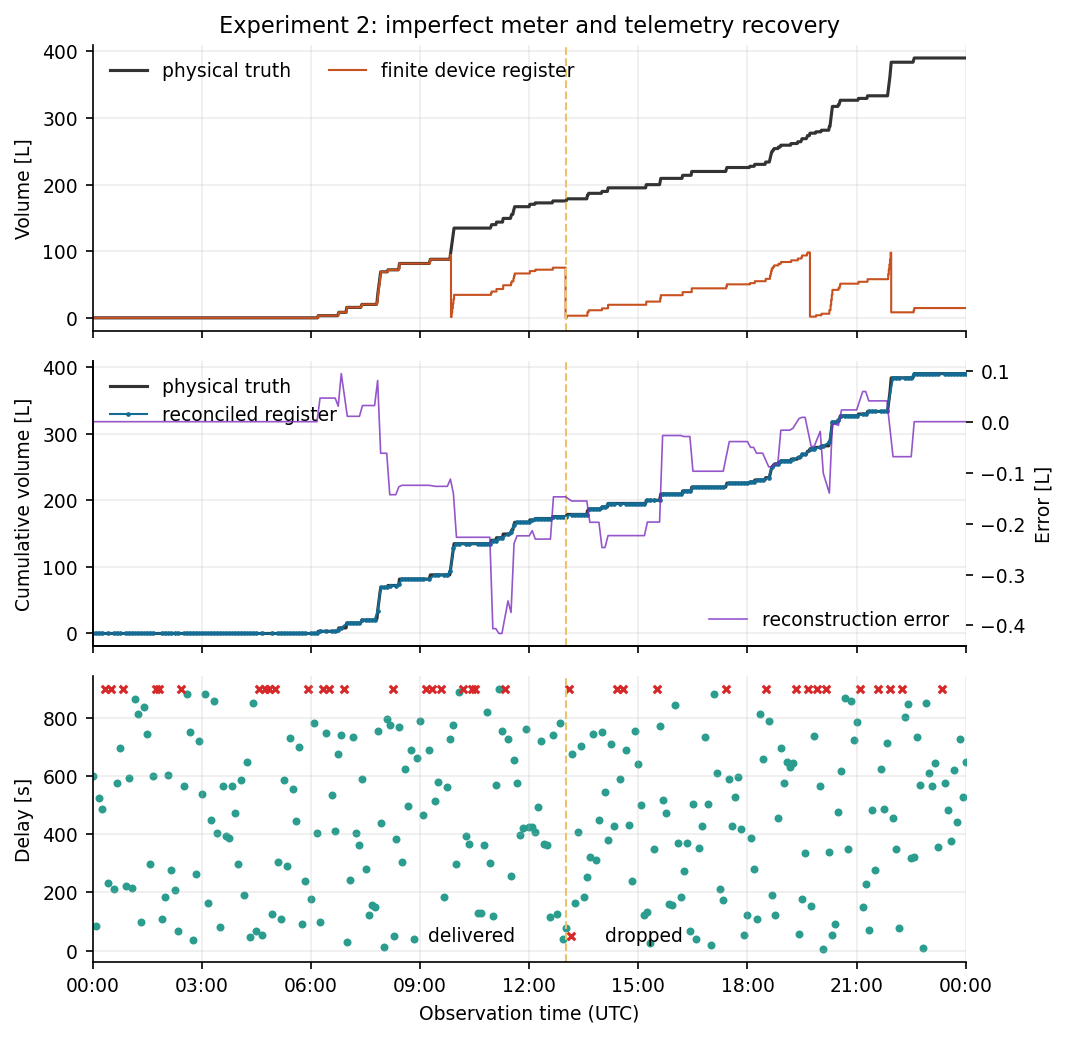
\includegraphics[width=0.86\linewidth]{experiment_2_telemetry_recovery.png}
  \caption{Experiment~2. Top: physical cumulative volume and the finite raw
  register; the dashed line marks the declared reset. Middle: reconciled
  cumulative volume and reconstruction error. Bottom: packet delay by
  observation time, with dropped packets marked by crosses.}
  \label{fig:experiment2}
\end{figure}

The maximum error of $0.416\,\mathrm{L}$ and RMSE of $0.124\,\mathrm{L}$ are
small relative to the $390\,\mathrm{L}$ daily total and satisfy the declared
limits. The nearly zero final error is a seed-specific cancellation after
increment noise and register quantization; it is not evidence that the meter is
unbiased. Likewise, one designed day cannot establish a statistical packet-loss
or reconstruction guarantee. A later sensitivity campaign should vary seeds,
loss bursts, readout intervals, noise levels, and modulus.

The reset result also depends on explicit protocol metadata. A silent reset is
not distinguishable in general from rollover or replacement using a single raw
register alone. Production ingestion should therefore retain device event
codes, meter identity and installation history, and reception timestamps
alongside the canonical observation. Experiment~2 validates that this metadata
can be kept outside the device-independent measurement payload without changing
its quantity, unit, or observation-time semantics.

\section{Iteration D: apartments and shared DHW storage}
Experiment~3 introduces the first building topology. Four independently seeded
apartments generate fixture demand, apartment meters feed an exact building
aggregator, and the combined hot-water branch draws from a shared, well-mixed
storage tank. The experiment returns to ideal meter transport so that topology
and storage dynamics can be isolated; composing the Experiment~2 telemetry
faults with this building is a later integration task.

\subsection{Apartment population and aggregation}
Each apartment reuses the Experiment~1 fixture shares and hot-water fraction,
but has its own occupancy, demand scale, and random seed. Both per-person total
and hot-water targets are multiplied by the same scale, preserving the
reference hot-water fraction. Table~\ref{tab:experiment3-apartments} states the
complete designed population.

\begin{table}[htbp]
  \centering
  \caption{Apartment assumptions and realized Experiment~3 totals.}
  \label{tab:experiment3-apartments}
  \begin{tabular}{lrrrrr}
    \toprule
    Apartment & Occupants & Scale & Events & Total [L] & Hot [L] \\
    \midrule
    101 & 1 & 0.80 & 17 & 104.0 & 36.0 \\
    102 & 2 & 1.00 & 38 & 260.0 & 90.0 \\
    201 & 3 & 1.10 & 60 & 429.0 & 148.5 \\
    202 & 4 & 0.90 & 66 & 468.0 & 162.0 \\
    \midrule
    Building & 10 & -- & 181 & 1261.0 & 436.5 \\
    \bottomrule
  \end{tabular}
\end{table}

For each branch $x\in\{\mathrm{tot},\mathrm{cold},\mathrm{hot}\}$, building
flow and volume are
\begin{equation}
  q_{x,\mathrm{bldg},k}=\sum_{a=1}^{N_a}q_{x,a,k},\qquad
  V_{x,\mathrm{bldg},k}=\sum_{a=1}^{N_a}V_{x,a,k}.
\end{equation}
The total branch must also satisfy
$q_{\mathrm{tot},\mathrm{bldg},k}=
q_{\mathrm{cold},\mathrm{bldg},k}+q_{\mathrm{hot},\mathrm{bldg},k}$.
This gives both pointwise and cumulative reconciliation checks. The coincidence
benefit is summarized by the diversity factor
\begin{equation}
  f_{\mathrm{div}}=
  \frac{\sum_a\max_k q_{\mathrm{tot},a,k}}
       {\max_k q_{\mathrm{tot},\mathrm{bldg},k}}.
\end{equation}

\subsection{Shared storage and boiler model}
The reference store contains $300\,\mathrm{L}$ of well-mixed water. Its
temperature state is represented by thermal energy above the cold-inlet
baseline,
\begin{equation}
  E_k=\rho c_p V_{\mathrm{tank}}
  \left(T_{\mathrm{tank},k}-T_{\mathrm{cold}}\right).
\end{equation}
At each one-minute step, the energy balance is
\begin{equation}
  E_{k+1}=E_k+
  \left(P_{\mathrm{boiler},k}-P_{\mathrm{DHW},k}
        -P_{\mathrm{loss},k}\right)\Delta t,
\end{equation}
where
\begin{align}
  P_{\mathrm{DHW},k}
    &=\rho c_p q_{\mathrm{hot},\mathrm{bldg},k}
      \left(T_{\mathrm{tank},k}-T_{\mathrm{cold}}\right),\\
  P_{\mathrm{loss},k}
    &=UA\max\left(T_{\mathrm{tank},k}-T_{\mathrm{amb}},0\right).
\end{align}
The assumptions are $T_{\mathrm{cold}}=10\,^{\circ}\mathrm{C}$,
$T_{\mathrm{amb}}=20\,^{\circ}\mathrm{C}$, and
$UA=3\,\mathrm{W\,K^{-1}}$. A hysteresis controller enables the boiler at
$55\,^{\circ}\mathrm{C}$ and disables it at $60\,^{\circ}\mathrm{C}$.
Thermal output is capped at $30\,\mathrm{kW}$ and plant input is
$P_{\mathrm{in}}=P_{\mathrm{boiler}}/0.90$. Power is reduced near the upper
energy bound to avoid numerical overheating.

\subsection{Acceptance criteria and verification}
Experiment~3 is accepted when (i) apartment branches aggregate exactly at every
step and at the cumulative registers, (ii) the building hot/cold split
conserves water, (iii) the tank balance closes including stored-energy change,
(iv) boiler input and thermal output satisfy the configured efficiency, (v)
tank temperature remains above $50\,^{\circ}\mathrm{C}$ and at or below
$60\,^{\circ}\mathrm{C}$, (vi) multiple apartments are active
simultaneously and the heater cycles, (vii) 56,180 canonical observations
round-trip through storage, and (viii) repeated runs are byte-identical.

The combined test suite now contains 25 passing tests. New checks cover exact
apartment targets, pointwise and cumulative aggregation, invalid duplicate
apartment identities, tank state and power bounds, the full energy balance, and
complete repeated-run output equality. CI regenerates Experiments~0--3 twice
and compares all machine-readable artifacts byte-for-byte.

\section{Experiment 3 results}
The four apartments produce 181 fixture events and
$1261.0\,\mathrm{L}$ of total water, including $436.5\,\mathrm{L}$ of hot
water. Table~\ref{tab:experiment3-results} summarizes the building and shared
plant result.

\begin{table}[htbp]
  \centering
  \caption{Experiment~3 building and shared-storage results.}
  \label{tab:experiment3-results}
  \begin{tabular}{lr}
    \toprule
    Metric & Result \\
    \midrule
    Building peak / sum of apartment peaks & 15.096 / 41.997 L/min \\
    Diversity factor & 2.782 \\
    Maximum simultaneously active apartments & 3 of 4 \\
    Minimum / weighted-mean / final tank temperature
      & 54.235 / 57.116 / 58.890 $^{\circ}$C \\
    Heater cycles / runtime & 12 / 58 min \\
    Peak DHW / boiler thermal power & 28.288 / 30.000 kW \\
    Delivered DHW energy & 23.808 kWh \\
    Standing loss & 2.756 kWh \\
    Boiler thermal output / plant input & 26.179 / 29.087 kWh \\
    Boiler conversion loss & 2.909 kWh \\
    Stored-energy change & $-0.385$ kWh \\
    Maximum water residual & $1.33\times10^{-15}\,\mathrm{m^3}$ \\
    Maximum energy residual & $8.94\times10^{-8}\,\mathrm{J}$ \\
    Canonical measurements / acceptance & 56,180 / pass \\
    \bottomrule
  \end{tabular}
\end{table}

The separate apartment peaks sum to $41.997\,\mathrm{L\,min^{-1}}$, but the
largest coincident building flow is only
$15.096\,\mathrm{L\,min^{-1}}$. Thus the realized building peak is 35.9\% of
the naive peak sum and $f_{\mathrm{div}}=2.782$. This is the first useful
system-level result: independently timed demands materially reduce the
simultaneous flow that the shared infrastructure sees.

Figure~\ref{fig:experiment3} shows how the same coincidence drives the storage
plant. The tank buffers the combined draws, falls below the $55\,^{\circ}$C
switch-on threshold during some one-minute intervals, and is reheated by twelve
boiler cycles. Its minimum temperature is $54.235\,^{\circ}$C, above the
declared $50\,^{\circ}$C service limit, while the volume-weighted supply
temperature is $57.116\,^{\circ}$C.

\begin{figure}[t]
  \centering
  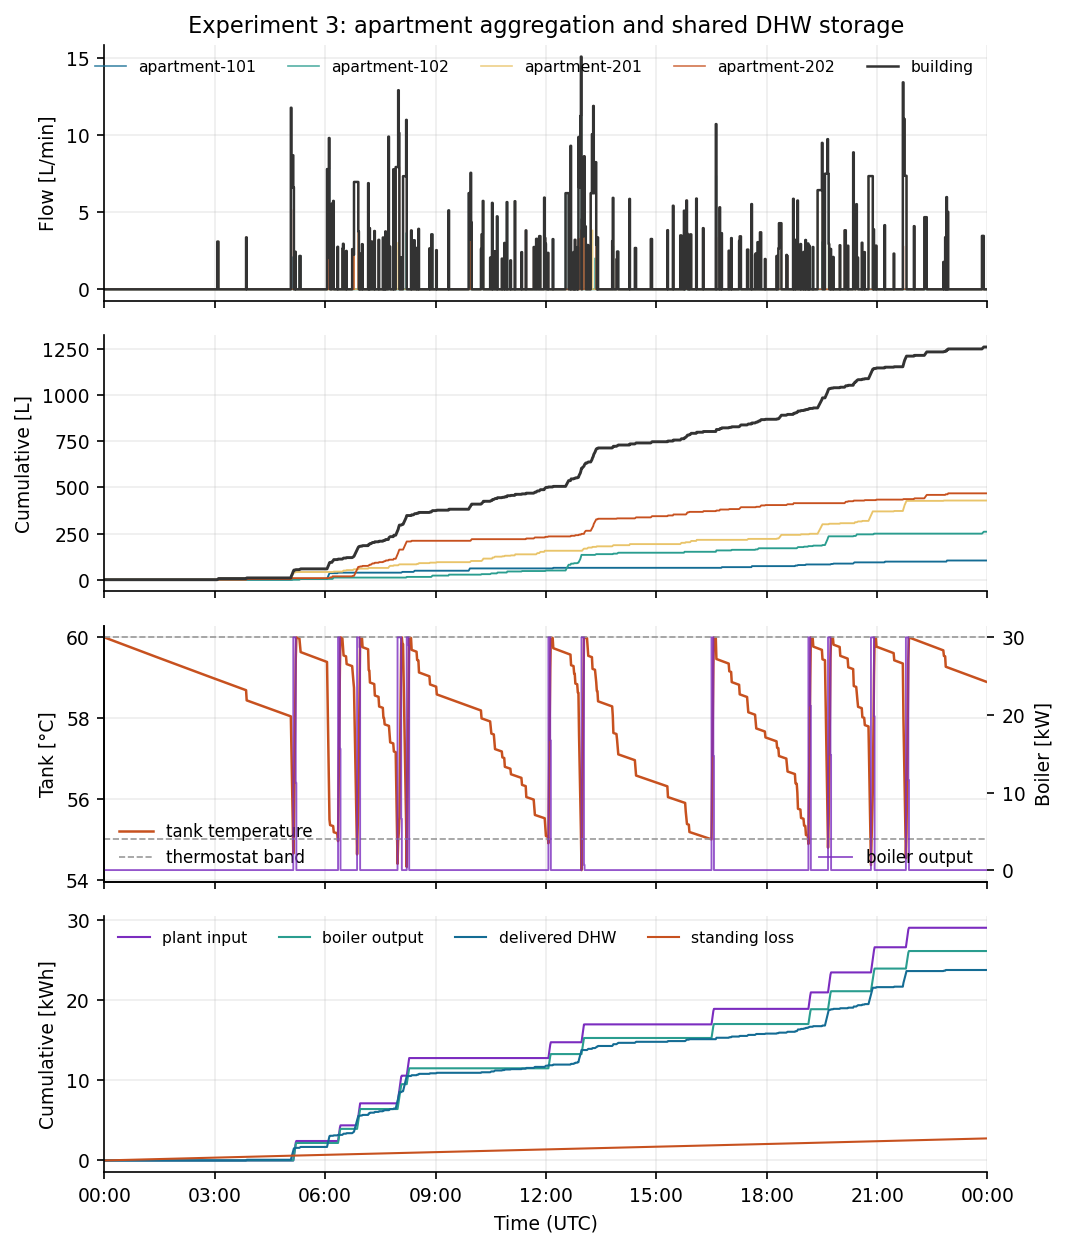
\includegraphics[width=0.84\linewidth]{experiment_3_building_storage.png}
  \caption{Experiment~3. From top to bottom: apartment and building flows;
  cumulative apartment contributions and building total; tank temperature,
  thermostat band, and boiler thermal output; cumulative plant input, boiler
  output, delivered DHW energy, and standing loss.}
  \label{fig:experiment3}
\end{figure}

The plant draws $29.087\,\mathrm{kWh}$. Of the $26.179\,\mathrm{kWh}$
thermal boiler output, $23.808\,\mathrm{kWh}$ reaches the hot-water branch and
$2.756\,\mathrm{kWh}$ is lost from storage. The tank ends
$0.385\,\mathrm{kWh}$ below its initial state, which closes the balance:
boiler output minus delivered energy and standing loss equals the stored-energy
change. Omitting this state term would make daily allocation appear inconsistent.

These values characterize one designed reference day, not a sizing study. The
apartment scales and fixture allocation are assumptions; daily totals are
normalized and day-to-day variation is absent. The tank is perfectly mixed;
pipe hydraulics, distribution temperature drop, recirculation, draw-off
stratification, and boiler transients are not modelled. Ideal apartment meters
also isolate Experiment~3 from the telemetry faults of Experiment~2. Multi-seed
and parameter sweeps are required before the diversity factor, cycling, or loss
fractions can support equipment or business decisions.

\FloatBarrier
\section{Iteration E: reconciliation and anomaly analytics}
Experiment~4 closes the previously separate topology and telemetry paths. The
four apartment total-water registers and the building register are now finite,
noisy devices with five-minute readout, independent packet loss and delay, and
rollover. The building meter also undergoes one declared reset. Reconciled
registers feed a water-balance detector, while the shared-tank state equation
feeds a thermal-loss detector. All detector inputs and residual outputs retain
the canonical measurement contract and are persisted through the file-backed
store.

This experiment is a controlled detectability study, not a trained anomaly
classifier. It asks whether known deviations remain visible after realistic
meter and transport imperfections, and whether the available measurements are
sufficient to attribute their cause.

\subsection{Injected reference anomalies}
Three non-overlapping four-hour deviations are introduced on the same reference
day:
\begin{enumerate}
  \item from 03:00 to 07:00 UTC, a constant
  $0.30\,\mathrm{L\,min^{-1}}$ leak is included by the building meter but not
  by any apartment meter, producing $72.0\,\mathrm{L}$ of unallocated water;
  \item from 11:00 to 15:00 UTC, apartment~201 registers only 75\% of its true
  increments, omitting $15.760\,\mathrm{L}$ over the realized demand trace;
  \item from 18:00 to 22:00 UTC, the tank standing-loss coefficient is four
  times its nominal value, adding $1.366\,\mathrm{kWh}$ of storage loss.
\end{enumerate}
The water windows do not overlap so each injection can be evaluated separately.
The detector itself receives no injection labels.

Each of the five water meters has $0.1\,\mathrm{L}$ resolution, 0.5\% standard
deviation on positive increments, a $200\,\mathrm{L}$ finite register, 8\%
packet-loss probability, and a uniformly sampled delay up to ten minutes.
Seeds are distinct across meters. First and final packets and the declared
building-meter reset are delivered by construction. Reconciliation is performed
offline in observation-time order; the result therefore tests data-quality and
diagnostic logic rather than the behavior of a real-time alarm service.

\subsection{Water-balance detector and identifiability}
Analytics uses successive timestamps that are available for the building meter
and all apartment meters. For a common window $[t_i,t_j]$, the volume and
average-rate residuals are
\begin{align}
  r^V_{ij}
    &= \Delta V_{\mathrm{bldg},ij}
       - \sum_{a=1}^{N_a}\Delta V_{a,ij},\\
  r^q_{ij} &= \frac{r^V_{ij}}{t_j-t_i}.
\end{align}
Missing packets lengthen a window rather than being interpreted as zero
consumption. The result becomes available only after the latest packet for its
end boundary has arrived. A water alarm is issued when
$|r^q_{ij}|\geq 0.15\,\mathrm{L\,min^{-1}}$.

The residual reveals an important structural limitation. Neglecting small
quantization and noise errors, the positive residual in this experiment is
\begin{equation}
  r^V_{ij}
  = V_{\mathrm{leak},ij}
    + (1-\alpha)\Delta V_{201,ij},
  \qquad \alpha=0.75.
\end{equation}
The same balance equation therefore observes both a downstream leak and an
under-registering apartment meter. With only one building register and the four
apartment registers, their sources are not identifiable from the residual
alone. Additional evidence such as night-flow persistence, valve state, a
redundant branch meter, meter self-diagnostics, or a maintenance test is needed
for attribution. Experiment~4 consequently reports the operational alarm as a
\emph{water-balance anomaly}, not as a confirmed leak.

\subsection{Thermal-loss detector}
The storage detector compares the measured tank-state change with the nominal
energy model over each five-minute window:
\begin{align}
  r^E_{ij}
    &= \Delta E_{\mathrm{tank},ij}
       - \left(\Delta E_{\mathrm{boiler},ij}
       - \Delta E_{\mathrm{DHW},ij}
       - \Delta E_{\mathrm{loss,nom},ij}\right),\\
  P_{\mathrm{unacc},ij} &= -\frac{r^E_{ij}}{t_j-t_i}.
\end{align}
Here the nominal loss uses the Experiment~3 coefficient
$UA=3\,\mathrm{W\,K^{-1}}$ and the simulated tank temperature. An alarm is
issued for $P_{\mathrm{unacc},ij}\geq150\,\mathrm{W}$. The physical simulator
continues to close its balance with the actual loss. The residual measures only
the mismatch between actual and nominal loss models.

\subsection{Acceptance criteria and verification}
Experiment~4 is accepted when all configured telemetry fault classes occur,
all register rollovers and the reset are recovered, and telemetry reconstruction
error remains below $1.0\,\mathrm{L}$. The water detector must identify both
injected events with precision at least 0.85 and recall at least 0.70. The
thermal detector must achieve precision and recall of at least 0.95. Finally,
all canonical raw, reconciled, and residual measurements must round-trip through
storage, and independent runs must produce byte-identical machine-readable
artifacts.

The complete suite now contains 31 passing tests. New unit tests cover anomaly
window validation, loss-multiplier bounds, unchanged nominal Experiment~3
behavior, multi-meter rollover/reset recovery, physical storage conservation,
water and thermal alarm behavior, and the deliberately unresolved water-source
ambiguity. The end-to-end runner is executed twice and compares the measurement,
telemetry, water-balance, thermal-balance, alarm, and summary files exactly.

\section{Experiment 4 results}
Table~\ref{tab:experiment4-results} summarizes the reference run. The five
meters schedule 1,445 packets and deliver 1,339. Packet loss leaves 197 adjacent
common water-balance windows rather than the 288 ideal five-minute windows.
All eleven rollovers and the single reset are recovered. The largest error of a
reconciled register relative to its intended device-level cumulative signal is
$0.468\,\mathrm{L}$.

\begin{table}[htbp]
  \centering
  \caption{Experiment~4 telemetry and anomaly-detection results.}
  \label{tab:experiment4-results}
  \begin{tabular}{lr}
    \toprule
    Metric & Result \\
    \midrule
    Water meters / scheduled / delivered packets & 5 / 1,445 / 1,339 \\
    Simulated and recovered rollovers / resets & 11 / 11; 1 / 1 \\
    Maximum telemetry reconstruction error & 0.468 L \\
    Common water windows & 197 \\
    Injected leak / omitted apartment volume & 72.0 / 15.760 L \\
    Water TP / FP / FN & 45 / 0 / 0 \\
    Water precision / recall & 1.000 / 1.000 \\
    Leak / meter-fault detection delay & 669 / 1,086 s \\
    Thermal TP / FP / FN & 48 / 0 / 0 \\
    Thermal precision / recall & 1.000 / 1.000 \\
    Peak unaccounted loss power & 359.204 W \\
    Excess standing loss / added plant input & 1.366 / 1.405 kWh \\
    Heater runtime, baseline / anomaly & 58 / 60 min \\
    Canonical measurements / alarms & 3,163 / 93 \\
    Acceptance & pass \\
    \bottomrule
  \end{tabular}
\end{table}

\FloatBarrier
Figure~\ref{fig:experiment4} shows that the reconciled water residual follows
the constant leak and the intermittent omitted apartment volume despite packet
loss, delayed arrivals, finite resolution, and device noise. The apartment~201
register error then remains near $-16\,\mathrm{L}$ because a cumulative meter
cannot recover volume that it never registered. The thermal residual changes
from numerical zero to approximately 330--359 W during the excess-loss window.

\begin{figure}[t]
  \centering
  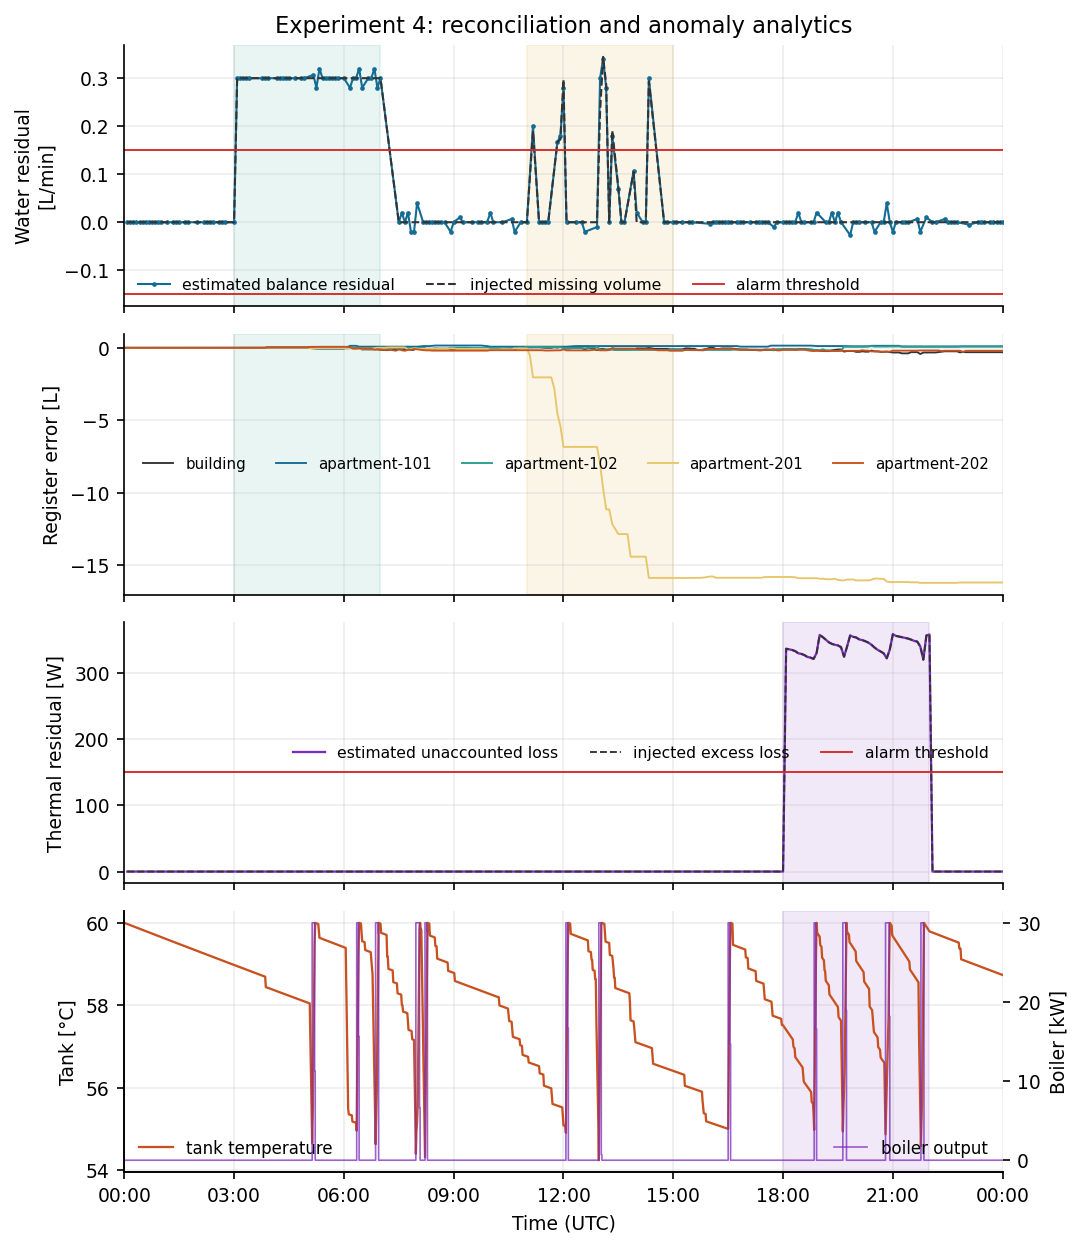
\includegraphics[width=0.88\linewidth]{experiment_4_anomaly_analytics.png}
  \caption{Experiment~4. Top: reconciled building-minus-apartment water
  residual, injected missing volume, and alarm threshold; second: reconciled
  register errors relative to physical volume; third: storage-model residual;
  bottom: tank temperature and boiler output. Green, amber, and violet bands
  mark the leak, meter under-registration, and excess-loss windows.}
  \label{fig:experiment4}
\end{figure}

Both detectors achieve perfect window-level scores on this designed day, but
this is a pipeline verification result rather than evidence of field-level
performance. The anomalies are large, non-overlapping, and evaluated using
thresholds chosen for this configuration. Only one physical demand seed and one
set of telemetry seeds are used. The thermal channels and model parameters are
known exactly except for the injected loss multiplier, and the detector has no
sensor drift, temperature bias, or boiler-state error to reject. Most
importantly, water-balance detection does not establish leak attribution. A
multi-day, multi-seed threshold study with smaller and overlapping anomalies is
needed before sensitivity, specificity, or detection delay can be generalized.

The useful conclusion is narrower and more concrete: the canonical data path
survives the combined building and telemetry complexity, volume and energy
residuals can expose controlled departures, and the experiment identifies which
business claim the present sensor topology cannot yet support.

\FloatBarrier
\section{Iteration F: external-file adapter substitution}
Experiment~5 tests whether a device-like external file can replace the simulated
measurement source without changing downstream contracts. The experiment starts
at the ingestion boundary: its runner never invokes the physical simulator,
virtual meter, telemetry generator, or register reconciler. Instead it performs
the following fixed path:
\begin{equation}
  \begin{aligned}
  \text{vendor CSV}&\rightarrow\text{CSV adapter}
  \rightarrow\text{canonical measurement}\\
  &\rightarrow\text{JSONL store}
  \rightarrow\text{water-balance analytics}.
  \end{aligned}
\end{equation}

\subsection{Source fixture and adapter contract}
No real building export was supplied for this iteration. The checked-in source
is therefore a \emph{frozen representative vendor-format fixture}, derived once
from the delivered and reconciled water-register evidence of Experiment~4. This
choice preserves known reference anomalies and missing-readout patterns while
introducing an independently parsed external representation. It is useful for
interface verification, but it is neither historical field data nor evidence of
field performance.

The fixture contains 1,339 readings from one building meter and four apartment
meters. It deliberately uses semicolon delimiters, German source headings,
naive local Europe/Vienna timestamps, decimal-comma numbers, litre registers,
vendor meter identifiers, and the status codes \texttt{OK} and
\texttt{GESCHAETZT}. A versioned JSON configuration maps source fields, meter
identifiers, roles, quality codes, timestamp semantics, and units. The adapter
normalizes timestamps to UTC, converts litres to canonical cubic metres, maps
quality to the shared vocabulary, and creates deterministic measurement IDs.

Input validation rejects missing columns, unknown meters or status codes,
invalid timestamps, non-finite or negative registers, non-monotonic series, and
conflicting readings for the same meter and timestamp. Exact duplicate rows are
accepted once with an explicit audit disposition. Every source row receives an
audit entry, and the configured SHA-256 digest pins the fixture used by the
acceptance run.

\subsection{Imported-data-only analysis and acceptance}
Water balance is calculated solely from persisted canonical register readings.
The adapter configuration assigns each asset either the building or apartment
role; the analysis intersects their observation timestamps and applies the same
successive-register equation used in Experiment~4. Missing timestamps lengthen
a window instead of becoming zero consumption. A window is marked suspect when
any start or end register has suspect quality, and an alarm is raised at
$|r^q_{ij}|\geq0.15\,\mathrm{L\,min^{-1}}$.

Reference periods are used only to score this controlled substitution test:
03:00--07:00 UTC for the unmetered leak and 11:00--15:00 UTC for apartment-meter
under-registration. Acceptance requires the input hash to match, every source
row to be converted, every register to remain monotonic, the canonical JSONL
round trip to preserve all imported and derived measurements, both reference
periods to be detected, no alarm outside those periods, and two independent
runs to produce byte-identical machine-readable artifacts.

The complete suite contains 35 passing tests. The new adapter tests cover local
time and decimal-comma conversion, litre-to-cubic-metre normalization, quality
mapping, exact deduplication, and rejection of unknown, negative, and conflicting
input. The end-to-end test executes the frozen import, storage, and analytics
path twice and compares its measurement, audit, balance, alarm, and summary
files byte-for-byte.

\section{Experiment 5 results}
All 1,339 source rows were accepted into canonical measurements. The five sparse
series yield 197 common balance windows ranging from five to 30 minutes. The
analysis adds one canonical residual measurement per window, so the store holds
1,536 records. Table~\ref{tab:experiment5-results} summarizes the run.

\begin{table}[htbp]
  \centering
  \caption{Experiment~5 adapter-substitution results.}
  \label{tab:experiment5-results}
  \begin{tabular}{lr}
    \toprule
    Metric & Result \\
    \midrule
    Source / accepted rows & 1,339 / 1,339 \\
    Water meters & 5 \\
    Canonical stored measurements & 1,536 \\
    Common windows / duration range & 197 / 5--30 min \\
    Good / suspect windows & 88 / 109 \\
    Alarm threshold / peak residual & 0.15 / 0.340 L/min \\
    Leak alarms / detection delay & 36 / 300 s \\
    Meter-fault alarms / detection delay & 9 / 600 s \\
    Alarms outside reference periods & 0 \\
    Input digest matched / acceptance & yes / pass \\
    \bottomrule
  \end{tabular}
\end{table}

\FloatBarrier
Figure~\ref{fig:experiment5} shows the source-substituted path. The imported
building and apartment registers retain their sparse observation pattern. Their
common-window volume increments agree outside the reference periods. During the
leak period the residual stays near $0.30\,\mathrm{L\,min^{-1}}$; during
under-registration it is intermittent because missing registered volume depends
on apartment~201 demand. Both exceed the unchanged threshold, with first-window
detection delays of five and ten minutes respectively.

\begin{figure}[t]
  \centering
  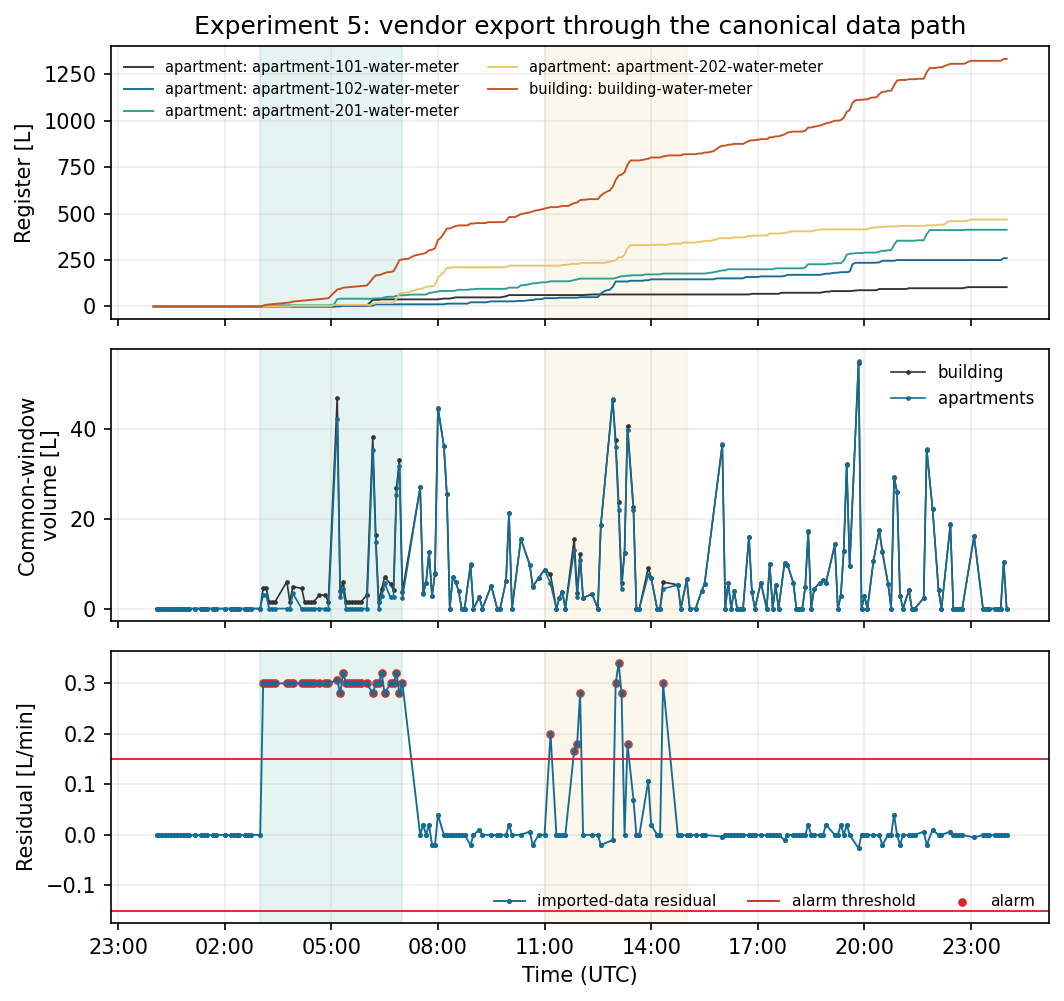
\includegraphics[width=0.90\linewidth]{experiment_5_file_adapter.png}
  \caption{Experiment~5. Top: cumulative water registers parsed from the
  vendor-format CSV; middle: building and summed-apartment volume over successive
  common windows; bottom: canonical-data water-balance residual and alarms.
  Green and amber bands mark the two controlled reference periods.}
  \label{fig:experiment5}
\end{figure}

The result supports the architectural claim that a configured external adapter
can replace the simulated source without changing canonical storage or the
balance algorithm. It does not validate operational performance on real meter
exports: the fixture is derived from a known simulation, contains one day and
one vendor layout, has no daylight-saving transition, and inherits the anomaly
sizes and threshold selected for Experiment~4. The aggregate residual also
retains the same identifiability limit: it signals missing volume but cannot
distinguish a leak from meter under-registration without additional evidence.

\FloatBarrier
\section{Pilot preparation P1: persistent backend}
Because authentic meter-system data are not yet available, the work after
Experiment~5 is separated into a pilot-preparation track. Experiment~6 remains
reserved for an unchanged, de-identified export from a physical meter system.
P1 instead asks whether the validated contracts can support a persistent
multi-building application backend and a stable interface for the planned
dashboard.

\subsection{Portfolio generator and relational model}
The P1 reference configuration represents 30 days at hourly boundaries for six
buildings, each containing 12 apartments. Apartment occupancy is seeded between
one and four people. A normalized diurnal profile, apartment-specific stochastic
variation, and a nominal consumption of 125 L per person and day generate the
cumulative registers. Building consumption is calculated as the exact sum of
its apartment increments before observation missingness is applied.

The generator emits the existing canonical cumulative-volume contract and adds
explicit portfolio, building, apartment, and meter topology. The reference case
contains 72 apartments and 78 meters. Apartment readings have a 2.5\% configured
missing probability, building readings 0.5\%, and all readings a 1.5\% suspect
quality probability. First and final boundaries are retained. These assumptions
exercise persistence and interface behavior; they are not estimates of real
fleet data quality.

P1 replaces experiment-local JSONL as the application store with a normalized
SQLite database. Separate tables hold schema metadata, portfolios, buildings,
apartments, meters, import jobs, and canonical measurements. Foreign keys encode
the topology, measurement identifiers remain the canonical primary keys, and
indexes support meter- and asset-time queries. SQLite provides a
zero-administration demonstration backend; PostgreSQL support and formal schema
migrations remain later product work.

\subsection{Idempotent loading and read API}
The portfolio configuration, topology, and canonical measurements define a
stable SHA-256 content digest. This digest produces a deterministic import ID.
The first load persists the topology and measurements in batches and records a
completed import. Replaying the same snapshot returns the existing import and
does not add data. A stored schema-version marker causes an explicit failure if
the application opens an incompatible database.

A FastAPI service exposes six routes: health, portfolio summary, building list,
meters for one building, time-ordered measurements for one meter, and import
history. The meter route supports bounded result size and optional time limits;
unknown buildings and meters return HTTP~404. Interactive OpenAPI documentation
is generated from the same application. P2 can therefore build the operator
dashboard against a stable API rather than directly reading experiment files.

Acceptance requires exact topology and measurement counts after persistence,
a complete first load, a zero-write replay in which every input measurement is
recognized as already stored, one auditable import, a complete building list in
the API snapshot, explicit schema-version agreement, and byte-identical summary
and API snapshots across independent runs. Eight new tests cover deterministic
generation, exact end-register aggregation, configuration validation,
persistence and query semantics, idempotency, incompatible schema rejection,
API success and error paths, and end-to-end reproducibility. The full suite now
contains 43 tests.

\section{Pilot P1 results}
The reference generator creates 54,917 canonical readings: 54,089 good and 828
suspect. The reduction from the 56,238 scheduled boundaries is caused by the
configured missingness. All generated topology and measurement records survive
the first database load. The second load accepts zero records and reports all
54,917 readings as duplicates under the same import ID. Table~\ref{tab:p1-results}
summarizes the frozen result.

\begin{table}[htbp]
  \centering
  \caption{Pilot-preparation P1 persistence results.}
  \label{tab:p1-results}
  \begin{tabular}{lr}
    \toprule
    Metric & Result \\
    \midrule
    Duration / resolution & 30 days / 60 min \\
    Buildings / apartments / meters & 6 / 72 / 78 \\
    Generated canonical measurements & 54,917 \\
    Good / suspect measurements & 54,089 / 828 \\
    First-load accepted / duplicate & 54,917 / 0 \\
    Replay accepted / duplicate & 0 / 54,917 \\
    Stored imports & 1 \\
    Read API routes & 6 \\
    Backend schema version & 1 \\
    Acceptance & pass \\
    \bottomrule
  \end{tabular}
\end{table}

\FloatBarrier
Figure~\ref{fig:p1} shows the six persisted building-level series summarized as
30-day volume and boundary completeness. Consumption differences follow the
seeded occupant mix and stochastic demand. Building-meter completeness remains
above 99\% for every building under the configured 0.5\% missing probability.

\begin{figure}[t]
  \centering
  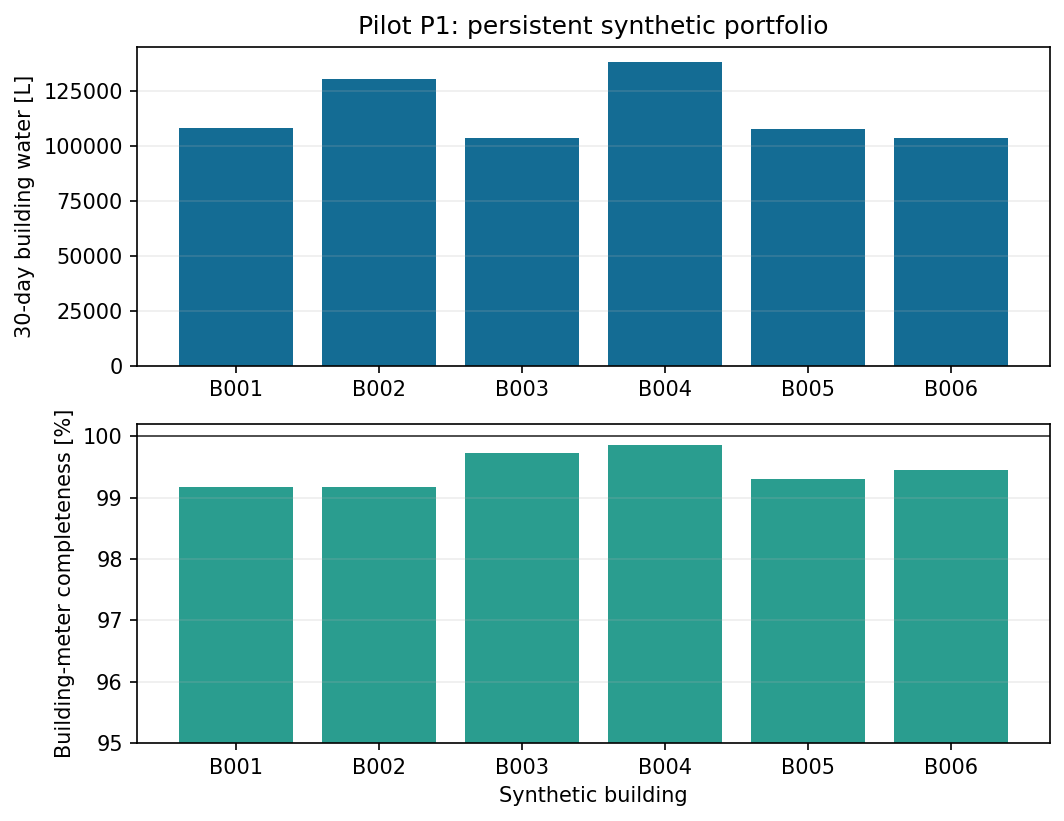
\includegraphics[width=0.88\linewidth]{pilot_p1_persistent_portfolio.png}
  \caption{Pilot P1. Top: 30-day cumulative water consumption of the six
  synthetic buildings; bottom: observed building-meter boundaries relative to
  the complete hourly schedule.}
  \label{fig:p1}
\end{figure}

P1 demonstrates that the canonical contracts can support an idempotent,
queryable multi-building backend and provides the data boundary needed by the
dashboard. It does not demonstrate production scale, concurrent ingestion,
PostgreSQL portability, access control, vendor semantics, or operational
analytics performance. The committed database is intentionally omitted because
it is regenerated from the versioned configuration; the compact summary and
figure are retained as evidence.

\FloatBarrier
\section{Pilot preparation P2: operator dashboard}
P2 asks whether the P1 application boundary is sufficient for a coherent
operator workflow before a real operator or field source is available. The
implementation is a replaceable Streamlit and Plotly client. It reads all
portfolio, building, meter, import, and review data through the versioned HTTP
API and never accesses SQLite directly. This separation is intentional: a later
web client can replace Streamlit without changing persistence or analytics.

\subsection{Operator surfaces and evidence model}
The interface contains five working surfaces. Portfolio health summarizes
consumption, building-meter completeness, quality, and review load. Building
balance compares the building register with the sum of apartment registers at
complete common boundaries. Meter detail exposes cumulative history, quality
markers, completeness, and a canonical-record sample. The import view retains
source digest and accepted, duplicate, and completion information. The review
queue filters evidence by status and building and lets an operator persist the
states open, investigating, or resolved together with a note.

P2 adds five API routes for portfolio overview, building balance, meter profile,
issue listing, and issue update; the application therefore exposes 11 routes in
total. Review records are an additive table in the versioned backend. Their
identifiers, detection time, severity, and evidence are deterministic. Operator
status, note, and update time are mutable audit fields.

The reference queue deliberately uses simple data-quality rules rather than
introducing P3 analytics early. A meter is queued if observed completeness is
below 97.5\% or if more than 2.0\% of its observed readings are suspect. An item
becomes a warning below 96.5\% completeness or above 2.5\% suspect share;
otherwise it is informational. Every item stores its observed, expected,
missing, and suspect counts together with the thresholds. These values are
chosen to exercise the workflow under the P1 missingness model. They are not
field-calibrated operating thresholds.

Water balance is kept semantically separate from diagnosis. The dashboard calls
the quantity a balance residual and states that it is evidence, not attribution
to a leak or meter fault. Period consumption uses the retained first and final
boundaries. The plotted register comparison uses only timestamps available for
the building meter and every apartment meter, which prevents unequal timestamp
sets from creating a spurious residual.

Acceptance requires all five surfaces to be present through the API contract,
all six buildings and the import audit to be visible, meter quality and common-
boundary balance evidence to be exposed, every queue item to carry its trigger
evidence, and review updates to survive a new database session. Error paths for
unknown resources and empty review updates must be explicit. The compact
dashboard snapshot and summary must be byte-identical across independent runs.

\section{Pilot P2 results}
The reference portfolio produces 35 active review items across 78 meters. Of
these, 28 are informational and seven are warnings. Low completeness triggers
29 items, elevated suspect share triggers nine, and three items satisfy both
conditions. This overlap confirms that the queue consolidates evidence by meter
rather than creating duplicate work items for separate quality symptoms.

The six building meters have 99.17--99.86\% completeness. Depending on the
building, 515--548 of 721 hourly boundaries are common to the building meter and
all 12 apartment meters. At those common boundaries the synthetic physical
identity is retained. The maximum absolute 30-day building-minus-apartment
period residual is $0.0002\,\mathrm{L}$, which is attributable to serialization
rounding and far below the explicit $0.01\,\mathrm{L}$ tolerance. Table~\ref{tab:p2-results}
summarizes the frozen result.

\begin{table}[htbp]
  \centering
  \caption{Pilot-preparation P2 operator-workflow results.}
  \label{tab:p2-results}
  \begin{tabular}{lr}
    \toprule
    Metric & Result \\
    \midrule
    Operator pages / API routes & 5 / 11 \\
    Buildings / meters / readings & 6 / 78 / 54,917 \\
    Active review items & 35 \\
    Informational / warning & 28 / 7 \\
    Completeness / suspect triggers & 29 / 9 \\
    Items satisfying both triggers & 3 \\
    Building-meter completeness range & 99.17--99.86\% \\
    Common boundaries per building & 515--548 \\
    Maximum absolute period residual & 0.0002 L \\
    Reproducible snapshot / acceptance & yes / pass \\
    \bottomrule
  \end{tabular}
\end{table}

\FloatBarrier
Figure~\ref{fig:p2} shows the first portfolio-health surface in a compact,
reproducible form. The interface puts the portfolio scale and review load in the
first viewport, then relates building consumption to meter completeness. The
amber review coloring indicates operator work, not diagnosed leakage.

\begin{figure}[t]
  \centering
  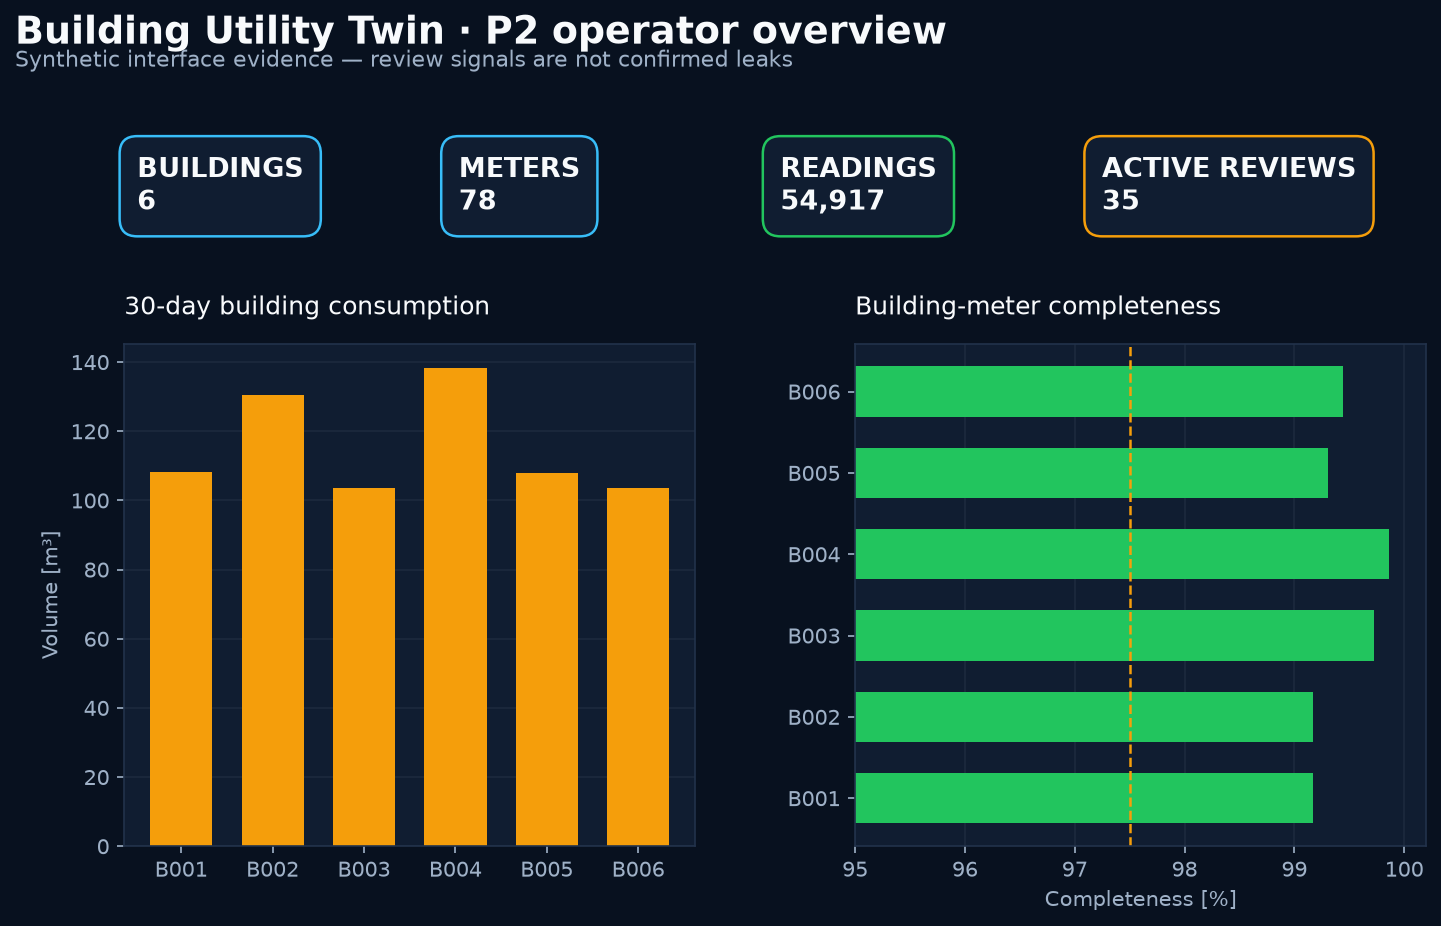
\includegraphics[width=0.96\linewidth]{pilot_p2_operator_overview.png}
  \caption{Pilot P2 operator overview for the deterministic six-building
  portfolio. The dashed line is the configured review threshold; it is an
  interface test value rather than a field-calibrated limit.}
  \label{fig:p2}
\end{figure}

A local in-process diagnostic over ten requests gave median response times of
approximately 0.94 s for the full portfolio overview, 0.14 s for one building
balance, 0.025 s for one meter profile, and 0.002 s for the issue list. These
figures are implementation diagnostics rather than portable benchmarks. They
show that the MVP is responsive at six-building scale while the overview's
repeated aggregation should be replaced by precomputed summaries or more direct
queries before a materially larger portfolio is claimed.

P2 connects persistent canonical readings to an evidence-backed operator
review. It does not validate whether the chosen
views match a property manager's workflow, whether the thresholds control false
alarms, or whether a residual identifies leakage. It also omits authentication,
multi-user concurrency, notification, deployment packaging, and accessibility
testing with representative users. Those omissions remain explicit inputs to
P3 and P5 rather than hidden assumptions.

\FloatBarrier
\section{Pilot preparation P3: analytics test bench}
P3 asks whether analytics with materially different evidential meanings can
share one persistence and interface boundary without implying the same level of
confidence. The implementation defines three explicit levels. Data-quality
evidence describes the integrity and timing of observations. Accounting and
plausibility evidence describes balances, completeness, and behavior that
merits investigation. Diagnostic-research evidence contains hypotheses or
model outputs that cannot be promoted to a diagnosis from this campaign.

\subsection{Evidence contract and campaign design}
Every analytic result has a deterministic evidence identifier, campaign and
analytic identifiers, evidence level, observed values, test thresholds,
provenance, expected and actual outcomes, interpretation, and an explicit
operational-claim permission. The possible outcomes are \texttt{clear},
\texttt{review}, and \texttt{research\_only}. The contract rejects a diagnostic-
research record unless its outcome is \texttt{research\_only}; it also rejects
any attempt to attach an operational claim to such a synthetic result.

The reference campaign covers the 14 mechanisms in the P3 plan. The six
data-quality cases independently inject one missing interval, a stale tail, one
duplicate row, one conflicting value, one register reversal, and a 15-minute
cadence shift into a complete reference register. The accounting and
plausibility cases calculate period consumption and inject an incomplete meter
topology, an unexplained 500 L building-register component, four persistent
night-flow windows, and 100 kWh of unaccounted thermal energy. The three
diagnostic cases retain two observationally equivalent causes for one water-
balance residual, fit a mean hourly consumption forecast, and fit an hourly
standardized anomaly score.

The interventions and thresholds are deliberately simple and visible. They
make each mechanism falsifiable in automated tests. They do not represent
estimated field prevalence, uncertainty, costs, or useful operating limits.
Table~\ref{tab:p3-levels} records the interface meaning of each level.

\begin{table}[htbp]
  \centering
  \caption{P3 evidence levels and permitted operator interpretation.}
  \label{tab:p3-levels}
  \begin{tabular}{p{0.30\linewidth}p{0.38\linewidth}p{0.20\linewidth}}
    \toprule
    Evidence level & Reference mechanisms & Permitted use \\
    \midrule
    Data quality & Integrity and timing checks & Clear or review \\
    Accounting / plausibility & Consumption and balances &
      Clear or review \\
    Diagnostic research & Attribution and fitted models & Research only \\
    \bottomrule
  \end{tabular}
\end{table}

\subsection{Persistence and operator boundary}
P3 adds idempotent campaign and evidence tables to backend schema version~2.
The first store accepts every evidence record. Replaying the same campaign
accepts none and reports every record as already present. Two new API routes
provide the campaign summary and filterable evidence, bringing the application
to 13 routes. A sixth dashboard page exposes coverage, outcomes, measured
values, and test thresholds.

The existing P2 review queue remains the action boundary. Only \texttt{review}
outcomes from data quality or accounting and plausibility are linked to an
operator issue. Clear results are retained as evidence but create no work.
Diagnostic-research records never enter the queue. The review view now handles
both the original completeness evidence and the richer P3 evidence without
changing status and note persistence.

\section{Pilot P3 results}
All 14 mechanisms produce their expected disposition. The evidence split is
six data-quality records, five accounting and plausibility records, and three
diagnostic-research records. The resulting outcomes are one clear, ten review,
and three research-only records. All ten review records, and only those
records, appear in the operator queue. The campaign makes zero operational
claims. Table~\ref{tab:p3-results} summarizes the frozen result.

\begin{table}[htbp]
  \centering
  \caption{Pilot-preparation P3 analytics-test-bench results.}
  \label{tab:p3-results}
  \begin{tabular}{lr}
    \toprule
    Metric & Result \\
    \midrule
    Analytics mechanisms & 14 \\
    Data quality / accounting / diagnostic & 6 / 5 / 3 \\
    Clear / review / research-only outcomes & 1 / 10 / 3 \\
    Expected mechanism agreement & 14 / 14 \\
    Operator issues created from P3 evidence & 10 \\
    First-load accepted / replay duplicate & 14 / 14 \\
    Dashboard pages / API routes & 6 / 13 \\
    Operational claims from synthetic campaign & 0 \\
    Reproducible snapshot / acceptance & yes / pass \\
    \bottomrule
  \end{tabular}
\end{table}

The data-quality interventions are isolated by construction. The missing,
duplicate, conflict, and reversal cases each expose one target event. The stale
case ends 7200 s before the analysis boundary, above the 5400 s test threshold.
Shifting one boundary by 15 minutes creates the expected two off-cadence
intervals.

The unmodified water-accounting endpoints retain a baseline residual of
$-0.0002\,\mathrm{L}$. Adding the 500 L intervention produces a
$499.9998\,\mathrm{L}$ residual and crosses the explicit 250 L test threshold.
Four night windows at $120\,\mathrm{L\,h^{-1}}$ cross the
$60\,\mathrm{L\,h^{-1}}$ threshold with three required consecutive windows.
The thermal case exposes 100 kWh of unaccounted energy against a 25 kWh test
threshold.

The mean-hour forecast uses 472 complete hourly training intervals and 236
synthetic holdout intervals. Its mean absolute error is
$13.076866\,\mathrm{L\,h^{-1}}$. The fitted hourly anomaly score ranks a 1000 L
injected hourly spike at 223.09, while the maximum ordinary synthetic holdout
score is 2.94. These values verify deterministic fitting, scoring, and holdout
separation for this intervention. They do not establish forecast skill or an
alarm operating point. The attribution case is more fundamental: the same
500 L residual is compatible with an unmetered leak or meter over-registration,
so the confirmed-cause count remains zero.

\FloatBarrier
Figure~\ref{fig:p3} shows the full campaign as it appears at the analytics
boundary. Amber records require review, green is a clear accounting result,
and purple denotes research that cannot be promoted to an operational claim.

\begin{figure}[t]
  \centering
  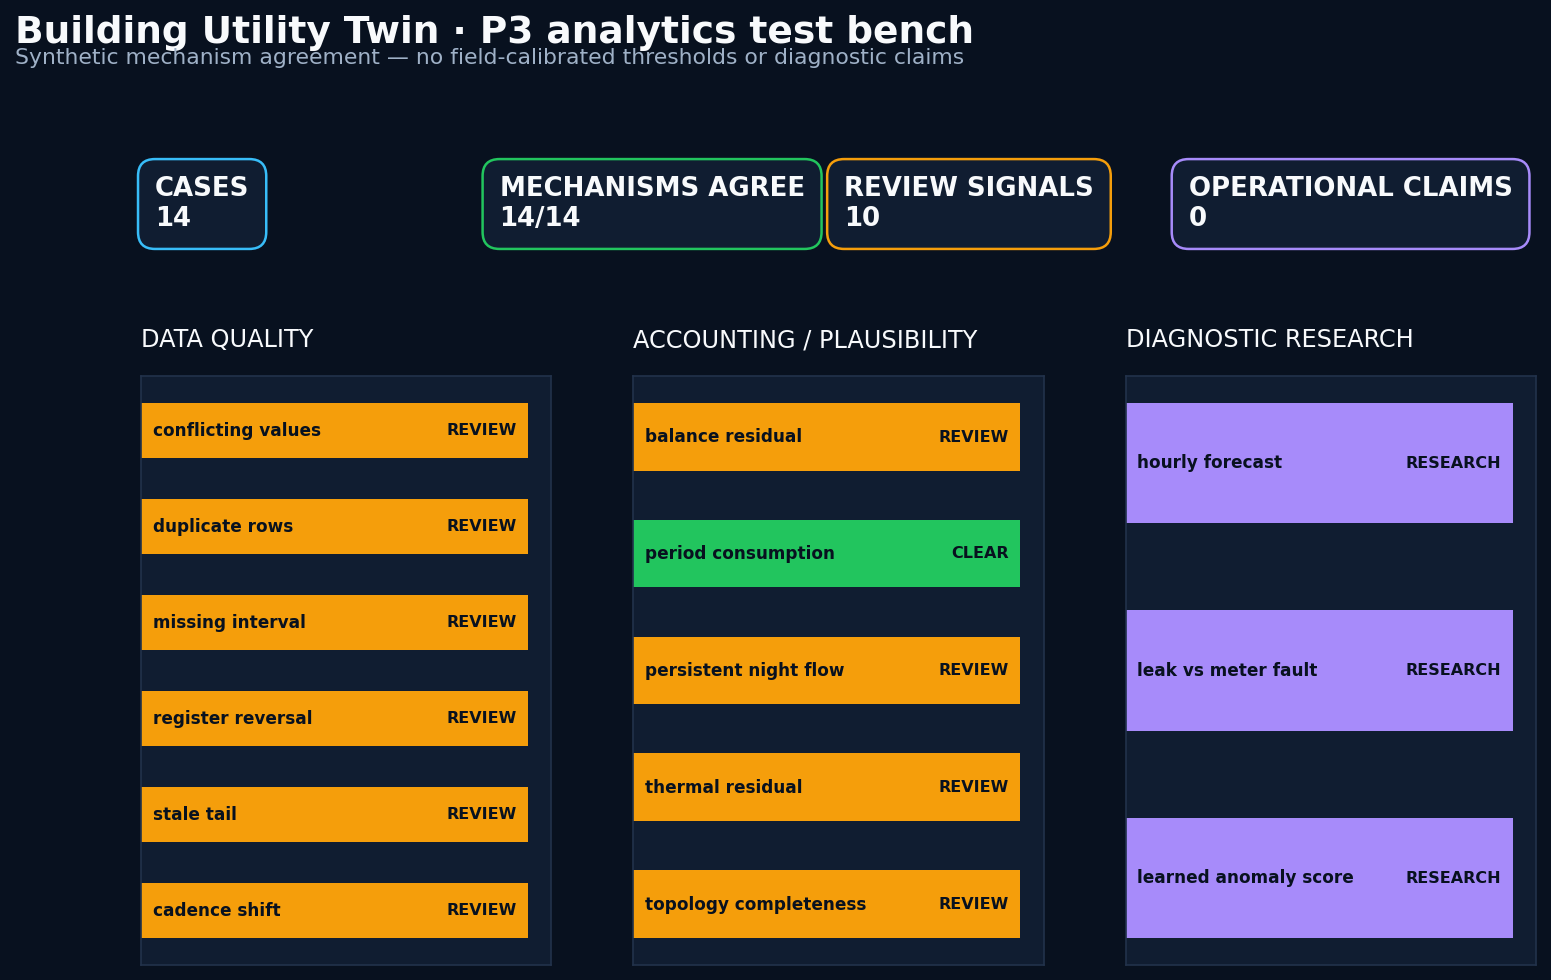
\includegraphics[width=0.98\linewidth]{pilot_p3_analytics_test_bench.png}
  \caption{Pilot P3 analytics test bench. The 14 synthetic cases agree with
  their expected software disposition while producing zero operational claims.}
  \label{fig:p3}
\end{figure}

The P3 result is a separation and integration result, not an accuracy result.
It demonstrates that evidence meaning survives computation, persistence, API
transport, operator presentation, and queue promotion. Two full independent
runs produce byte-identical analytics snapshots and summaries. Six new tests
raise the complete suite to 55 tests and cover the evidence contract,
determinism, persistence, idempotency, filtering, API validation, queue linkage,
and end-to-end reproducibility.

P3 does not validate useful thresholds, false-positive or false-negative rates,
seasonal forecast performance, uncertainty calibration, or diagnostic
attribution. The strongest finding is therefore the enforced boundary: even a
large synthetic score remains research-only until a separately selected
baseline and held-out physical data support an operational interpretation.

\FloatBarrier
\section{Planned extensions}
P4 will generalize the Experiment~5 vendor-adapter toolkit into declarative
mappings, import preview, conformance tests, version recognition, templates,
and a scaffold for new vendors. P5 will package the demonstrator with
operational safeguards.

Experiment~6 begins only when a real source is available. It should process an
unmodified, de-identified physical meter export and record its format version,
timezone, unit semantics, counter lifecycle, missingness, and calibration
metadata. A separate baseline period must select thresholds before held-out
evaluation. A real pilot must also define the additional evidence required to
distinguish leaks from meter errors.

\clearpage
\begingroup
\raggedright
\bibliographystyle{plain}
\bibliography{references}
\endgroup

\end{document}
